\documentclass{beamer}

\usepackage{amsmath}
\usepackage{amssymb}
\usepackage{booktabs}
\usepackage{rotating}
\usepackage{multirow}
\usepackage{colortbl,color}
\usepackage{graphics}

\usepackage{colortbl,color}
\usetheme{material}
\useLightTheme
\usePrimaryRed
\useAccentGreen

\renewcommand{\theenumii}{\alph{\enumii}}
\defbeamertemplate{itemize subitem}{dash}{--}
\defbeamertemplate{itemize subsubitem}{dash}{--}
\setbeamertemplate{itemize item}[circle]
\setbeamertemplate{itemize subitem}[dash]
\setbeamertemplate{itemize subsubitem}[dash]
\setbeamertemplate{enumerate item}{\arabic{enumi}.}
\setbeamertemplate{enumerate subitem}{(\alph{enumii})}
\usefoottemplate{}

\setbeamertemplate{headline}{}
\usenavigationsymbolstemplate{}


\newcommand{\SD}[1]{{\tiny $\left(#1\right)$}}
\newcommand{\SDm}[1]{{\tiny \left(#1\right)}}
\newcommand{\Prob}[1]{\mbox{Pr}\left\{#1\right\}}
\newcommand{\CProb}[2]{\mbox{Pr}\left\{#1\left|#2\right.\right\}}

\usepackage{array}
\newcolumntype{P}[1]{>{\centering\arraybackslash}p{#1}}

%\setbeamercovered{transparent}

\begin{document}
\section{Intro}
\title{\LARGE Econ 2220: Experimental Economics \\ Communication 1}
\author{Alistair J. Wilson }
\date{Fall 2020}
 \maketitle

\begin{frame}{Communication Intro}

	\begin{card}
    Communication:
		\begin{enumerate}
			\item Coordination
			\item Strategic Argumentation
			\item Analogy \& Instruction
		\end{enumerate}
	\end{card}
\end{frame}

\begin{frame}{Coordination}
	\begin{card}
	When there are multiple equilibria, how do we resolve this?
		\begin{itemize}
			\item In many situtations, applied theorists would select a particular equilibrium as being focal
			\item Experiments have been used to look for behavioral regularities in equilibrium selection
			\item Here we'll look at the effects of a potentially powerful device for coordination: communication.
		\end{itemize}
	\end{card}
\end{frame}

\begin{frame}{Cheap Talk (Farrell \& Rabin JEP 1996)}
    \begin{card}
    	\begin{itemize}
    		\item Broad overview article on the theory of communication and cheap talk
    		\item Outline natural language as a coordination device
    	\end{itemize}
    \end{card}
    \begin{card}
	Define some terms:
		\begin{itemize}
			\item Self-committing
			\item Self-signaling
		\end{itemize}
	\end{card}
\end{frame}


\begin{frame}
\begin{card}[Self-committing:]
		\begin{itemize}
			\item This is when the message, if it succeeds in persuading the other players, makes it optimal to take the advocated action
			\item For example: Any message which has other players follow the Nash Equilibrium is necessarily self-committing.
		\end{itemize}
\end{card}
\end{frame}

\begin{frame}
\begin{card}[Self-signaling]
		\begin{itemize}
			\item The message action induces behavior in others (if believed) that is optimal for the sender \textbf{if and only if} the sender takes the action she is advocating.
			\item For example: Coordination in a Battle of the Sexes Game 
		\end{itemize}
\end{card}
\end{frame}

\begin{frame}{Multiple Equilibria...}
    \begin{card}
    	\begin{itemize}
    		\item Note that the Stag-hunt game (and therefore the repeated PD) is not self-signaling!
    		\item Those hunting Hares would also prefer the other agent to choose to hunt a Stag
    		\item So a message of ``Let's Hunt Stag'' is \emph{self-committing}, but not \emph{self-signaling}
    		\item A message of ``Let's Hunt hare'' is both \emph{self-committing} and \emph{self-signaling}
    	\end{itemize}
    \end{card}
\end{frame}

\begin{frame}{Coordination}
	\begin{itemize}
		\item We will look at two types of coordination. Games in which the equilibria are :
		\begin{itemize}
			\item not Pareto-ranked (think Battle of the Sexes)
			\item Pareto-ranked (think Stag-hunt)
		\end{itemize}
	\end{itemize}
\end{frame}


\begin{frame}{Battle of the Sexes}
\begin{card}
From Cooper, DeJong, Forsythe and Ross (Rand 1989).
\begin{center}
Payoff Table $(x>y>0)$:

		\begin{tabular}{r|c|c|}
				\multicolumn{1}{r}{}& \multicolumn{1}{c}{$c_1$}  & \multicolumn{1}{c}{$c_2$} \\ \cline{2-3}
				$r_1$ &  $0,0$ & $y,x$ \\ \cline{2-3}
				$r_2$ &  $x,y$ & $0,0$ \\ \cline{2-3}
				\end{tabular}
\end{center}
\end{card}
	\begin{card}
This has three equilibria:
			\begin{itemize}
				\item $(r_1,c_2)$
				\item $(r_2,c_1)$
				\item Mixed strategy: $\tfrac{x}{x+y}$\% on strategy 2.
			\end{itemize}
	\end{card}
\end{frame}

\begin{frame}{Battle of the Sexes (Rand 1989)}
\begin{card}
	\begin{itemize}
		\item Think of this as an entry game
		\item Two firms, in a nearby industry have to decide whether to enter a new industry
		\item But, the new industry is a natural monopoly
		\item Each prefers that they be the monopolist, but both entering, or neither entering are the worst outcomes
		\item But if we think of firms as entirely symmetric, it seems strange to focus on the efficient asymmetric outcomes
	\end{itemize}
\end{card}
\end{frame}

\begin{frame}{Battle of the Sexes (Rand 1989)}
\begin{card}
	\begin{itemize}
		\item If we actually think of the choice of a couple deciding where to go, then it's obvious that communication is involved 
		\item But, even in the entry game example, announcements of intent, \emph{etc.} seem like they would do the same thing \pause
		\item Communication can serve to provide a public randomization device to allow for correlated equilibria.
	\end{itemize}
\end{card}	
\end{frame}

\begin{frame}{Battle of the Sexes (Rand 1989)}
    \begin{card}
    	\begin{itemize}
    		\item Suppose each player has two messages $\diamond$ and $\circ$
    		\item Think of the communication between each player as a simultaneous choice
    		\item As in the matching pennies game, let $(\diamond,\diamond)$ and $(\circ,\circ)$  mean that \emph{Row} enters
    		\item If the messages are $(\diamond,\circ)$ or $(\circ,\diamond)$ then \emph{Col} enters
    	\end{itemize}
    \end{card}
\end{frame}

\begin{frame}{Battle of the Sexes (Rand 1989)}
\begin{card}
	\begin{itemize}
		\item But this seems a little like the initial problem...
		\item Why would we assume two actors who were unable to coordinate on an equilibrium are suddenly able to coordinate on this communication pre-game?
		\item Natural language is a much more focal idea 
		\item So each instead will send a message for one option
	\end{itemize}
\end{card}
\end{frame}

\begin{frame}{Battle of the Sexes (Rand 1989)}
\begin{card}
	\begin{itemize}
		\item Maybe one player gets to move first, and therefore can credibly signal that they will enter
		\item In this sense, one player is asymmetric, and has the power to make one of the equilibria focal
	\end{itemize}
\end{card}		
\end{frame}

\begin{frame}{Battle of the Sexes (Rand 1989)}
\begin{card}
	\begin{itemize}		
		\item Or if the announcements are simultaneous, this is more like bargaining...
		\item With a back and forth conversation, this is somewhat like deciding to relent or not and go with the other's preferred option
		\item But this decision to relent is inherently strategic
		\item More rounds of the debate might be better, but more rounds also alters the behavior
	\end{itemize}
\end{card}
\end{frame}

\begin{frame}{Farrel (1987)}
\begin{card}
	\begin{itemize}
		\item Suppose there are $2$ periods of arguing. 
		\item In each period, the two players simultaneously send a message \emph{``Enter''}, \emph{``Stay Out''} or \emph{``Silence''}.
		\item Coordinated outcomes are:
	\end{itemize}
	\begin{center}
		\begin{tabular}{r|c|c|c|}
				\multicolumn{1}{r}{}& \multicolumn{1}{c}{\emph{Enter}}  & \multicolumn{1}{c}{\emph{Silence}} & \multicolumn{1}{c}{\emph{Stay Out}}\\ \cline{2-4}
				\emph{Enter} &  Mixed & Row  & Row \\ \cline{2-4}
				\emph{Silence} &  Column & Mixed &  Row\\ \cline{2-4}
				\emph{Stay Out} &  Column & Column & Mixed  \\ \cline{2-4}
    	\end{tabular}
    \end{center}
\end{card}
\end{frame}

\begin{frame}{Farrell (1987)}
    \begin{card}
    	\begin{itemize}
    		\item In the last period we can solve for indifference over each message using the Mixed outcome payoff $u=\tfrac{xy}{x+y}$
    		\item So the expected payoff in period $T$ is $V_T$\pause
    		\item In period $T-1$, the expected payoff from matched messages is $V_T$, so we can now work out the strategies and $V_{T-1}$\pause
    		\item So this is like bargaining, with an increasing probability of relenting as we get closer to the final outcome
    	\end{itemize}
    \end{card}
\end{frame}

\begin{frame}
	\begin{card}[Experimental Details (Cooper et al)]
		\begin{itemize}
			\item Undergrads and MBAs from University of Iowa
			\item 11 subjects in a session
			\begin{itemize}
				\item Everyone plays everyone else once
				\item One player sits out every round
			\end{itemize}
			\item Lottery method in every round for prizes (\$1 or \$2)
			\item $x=600$, $y=200$ ($\Longrightarrow u=150, \Pr\left\{\text{Eqbm}\right\}$) 
			\item First 10 periods play a dominant-strategy game
			\item Then twenty periods of treatment BoS game
		\end{itemize}
	\end{card}
\end{frame}

\begin{frame}
	\begin{card}[Treatments (Cooper et al.)]
		\begin{itemize}
			\item No Communication
			\item One-way communication
			\item Two-way communication (1 round)
			\item Two-way communication (3 rounds)
		\end{itemize}
		\end{card}
\begin{card}		
\textbf{Main assessment metric:} fraction of (pure) equilibrium outcomes
	\end{card}
\end{frame}

\begin{frame}{Battle of the Sexes (Rand 1989)}
	\begin{card}
		Data pooled across sessions
        
        	\begin{center}
        		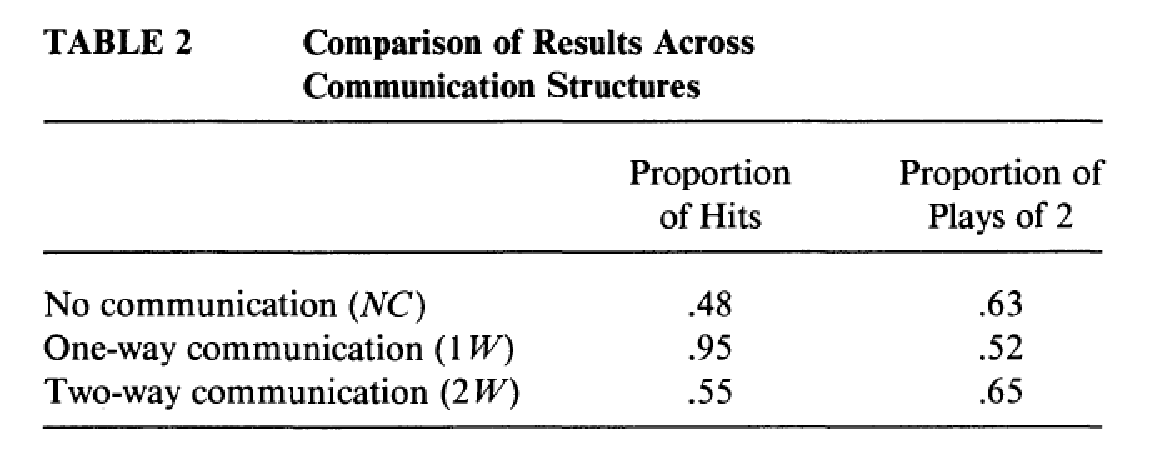
\includegraphics[width=0.9\textwidth]{./i/cdfr1989Tbl2.eps}
        	\end{center}
        \end{card}
        \begin{card}
		\begin{itemize}
			\item Baseline Hits in Mixed Eqbm is 0.375
			\item In Farrell model with one two-way round 0.499
		\end{itemize}
		\end{card}
\end{frame}

\begin{frame}{Battle of the Sexes (Rand 1989)}
	\begin{card}
	One-way communication:
    
    	\begin{center}
    		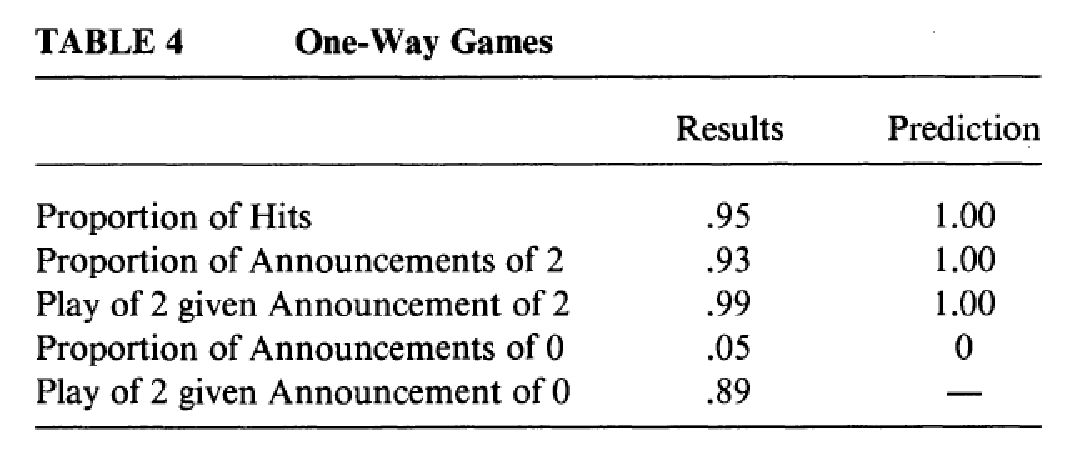
\includegraphics[width=0.9\textwidth]{./i/cdfr1989Tbl4.eps}
    	\end{center}
	\end{card}
\end{frame}

\begin{frame}{Battle of the Sexes (Rand 1989)}
	\begin{card}
	Two-way communication:

	\begin{center}
		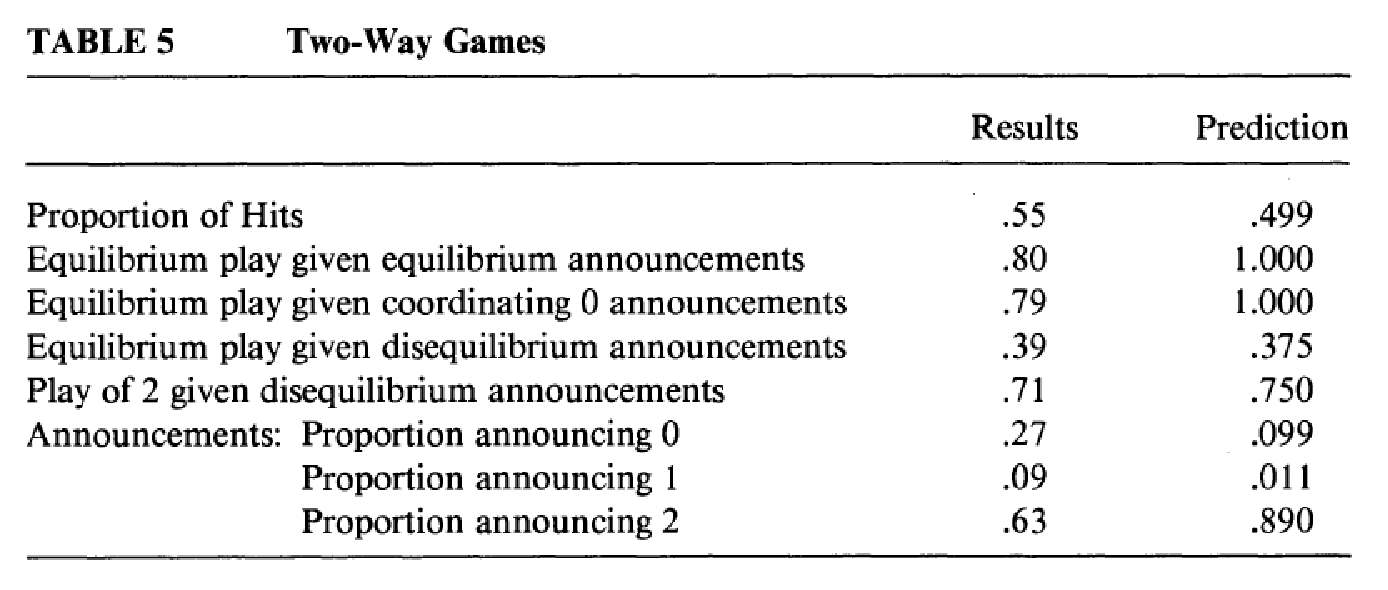
\includegraphics[width=0.9\textwidth]{./i/cdfr1989Tbl5.eps}
	\end{center}
	\end{card}
\end{frame}
\begin{frame}{Battle of the Sexes (Rand 1989)}
	\begin{card}
	Two-way communication with three rounds:

	\begin{center}
		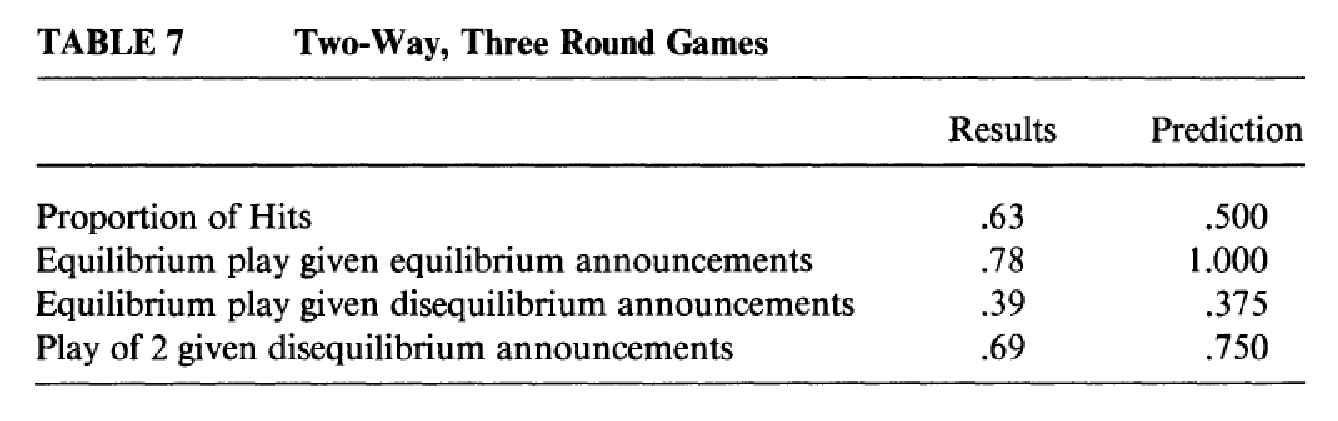
\includegraphics[width=0.85\textwidth]{./i/cdfr1989Tbl7.eps}
	\end{center}
	\end{card}
	
	\begin{card}
    	\begin{itemize}
    		\item Additional 2 rounds predicted to have only marginal effect, but still not as 
    		\item Small increase in Hits observed, up to 0.63 from 0.55, but not close to one way
    	\end{itemize}
    \end{card}
\end{frame}

\begin{frame}{Battle of the Sexes (Rand 1989)}
	\begin{card}[Conclusions]
		\begin{itemize}
			\item Assigning communication power to one individual much more efficient than two-way communication
			\item Focality via communication (as opposed to Schelling)
			\item Extra rounds do slightly better than predicted
			\item Broadly in line with the theory on two-way communication
		\end{itemize}
		\end{card}
	\begin{card}
	 For me a lot of the details are hidden. Focus is on the efficiency, would like to learn more about individual behavior
	\end{card}
\end{frame}

\begin{frame}{Pareto-ranked Equilibria}
    \begin{card}
    	\begin{itemize}
    		\item One refinement often used by theorists when dealing with multiple equilibria is to choose the Pareto-superior outcome
    		\item But thinking of the stag-hunt game, it is clear that other concerns might dominate (see Harsanyi \& Selten 1988)
    		\item Cooper et al. (AER 1990) experimentally demonstrate that coordination at the Pareto-superior equilibrium is not a sure thing
    		\begin{itemize}
    			\item Risk-dominance (Schmidt, Shupp, Walker and Ostrom GEB 2003)
    			\item Optimization-premium effects ( Battalio et al 2001.) 
    			\item But payoffs from dominated strategies can also effect coordination
    		\end{itemize}
	\end{itemize}
	\end{card}
\end{frame}

\begin{frame}{Equilibria Selection: Risk Dominance }
\begin{card}
\begin{center}
\begin{tabular}{r|c|c|}
				\multicolumn{1}{r}{}& \multicolumn{1}{c}{$Y_1$}  & \multicolumn{1}{c}{$Y_2$} \\ \cline{2-3}
				$X_1$ &  $45,45$ & $0,35$ \\ \cline{2-3}
				$X_2$ &  $35,0$ & $40,40$ \\ \cline{2-3}
\end{tabular}
\ \ vs. \ 
\begin{tabular}{r|c|c|}
				\multicolumn{1}{r}{}& \multicolumn{1}{c}{$Y_1$}  & \multicolumn{1}{c}{$Y_2$} \\ \cline{2-3}
				$X_1$ &  $45,45$ & $0,25$ \\ \cline{2-3}
				$X_2$ &  $25,0$ & $5,5$ \\ \cline{2-3}
\end{tabular}
\end{center}
\end{card}

\begin{card}
First game requires a confidence of 80\% or above on strategy 1. Second game only requires 20\%.
\end{card}
\end{frame}

\begin{frame}{Equilibria Selection: Optimization Premium (cf. Battalio et al EMA 2001)}
\begin{card}
\begin{center}
\begin{tabular}{r|c|c|}
				\multicolumn{1}{r}{}& \multicolumn{1}{c}{$Y_1$}  & \multicolumn{1}{c}{$Y_2$} \\ \cline{2-3}
				$X_1$ &  $45,45$ & $0,35$ \\ \cline{2-3}
				$X_2$ &  $35,0$ & $40,40$ \\ \cline{2-3}
\end{tabular}
\ \ vs. \ 
\begin{tabular}{r|c|c|}
				\multicolumn{1}{r}{}& \multicolumn{1}{c}{$Y_1$}  & \multicolumn{1}{c}{$Y_2$} \\ \cline{2-3}
				$X_1$ &  $45,45$ & $0,42$ \\ \cline{2-3}
				$X_2$ &  $42,0$ & $12,12$ \\ \cline{2-3}
\end{tabular}
\end{center}
\end{card}

\pause 

\begin{card}
More people choose $X_1$/$Y_1$ in second game, even though both games require 80\% chance other plays strategy $Y_1$)
\end{card}
\end{frame}

\begin{frame}{Equilibria Selection: With a Dominated Strategy}
\begin{card}
	\begin{center}{\footnotesize 
		\begin{tabular}{r|c|c|c|}
			\multicolumn{1}{r}{ }& \multicolumn{1}{c}{$Y_1$}  & \multicolumn{1}{c}{$Y_2$} & \multicolumn{1}{c}{$Y_3$} \\ \cline{2-4}
			$X_1$ &  $35,35$  & $35,25$  & $100,0$ \\ \cline{2-4}
			$X_2$ &  $25,35$  & $55,55$  & $0,0$   \\ \cline{2-4}
			$X_3$ &  $0,100$  & $0,0$    & $60,60$  \\ \cline{2-4}
		\end{tabular}\ vs\ \begin{tabular}{r|c|c|c|}
			\multicolumn{1}{r}{ }& \multicolumn{1}{c}{$Y_1$}  & \multicolumn{1}{c}{$Y_2$} & \multicolumn{1}{c}{$Y_3$} \\ \cline{2-4}
			$X_1$ &  35,35 & 35,25  & 100,0 \\ \cline{2-4}
			$X_2$ &  25,35 & 55,55  & 0,0 \\ \cline{2-4}
			$X_3$ &  0,100 & 0,0  & 50,50  \\ \cline{2-4}
		\end{tabular}
		}
	\end{center}
\end{card}	
\begin{card}Example form Cooper et al. (AER 1990)

 Removing the cooperative max point allows for greater coordination on the Pareto-dominant Nash equilibrium
\end{card}
\end{frame}

\begin{frame}{Communication and coordination in Pareto-ranked games}
	\begin{card}
 Cooper et al. (QJE 1992) examine the effect of cheap-talk communication on these games. Categorize these games in two ways:
			\begin{itemize}
				\item Simple coordination games (SCG)
				\item Cooperative coordination games (CCG)
			\end{itemize}
 By SCG they mean Stag-hunt type-games, and by CCG those games with a non-equilibrium cooperative outcome
	\end{card}
\end{frame}

\begin{frame}{Cooper et al. (QJE 1992)}
	\begin{card}
 SCG game is:
		\begin{center}
		\begin{tabular}{r|c|c|}
				\multicolumn{1}{r}{}& \multicolumn{1}{c}{$Y_1$}  & \multicolumn{1}{c}{$Y_2$} \\ \cline{2-3}
				$X_1$ &  $800,800$ & $800,0$ \\ \cline{2-3}
				$X_2$ &  $0,800$ & $1000,1000$ \\ \cline{2-3}
\end{tabular}
\end{center}
\end{card}
\begin{card}CCG game is:
		\begin{center}
			\begin{tabular}{r|c|c|c|}
				\multicolumn{1}{r}{ } & \multicolumn{1}{c}{$Y_1$}  & \multicolumn{1}{c}{$Y_2$} & \multicolumn{1}{c}{$Y_3$} \\ \cline{2-4}
				$X_1$ &  350,350 & 350,250  & 1000,0 \\ \cline{2-4}
				$X_2$ &  250,350 & 550,550  & 0,0 \\ \cline{2-4}
				$X_3$ &  0,1000 & 0,0  & 600,600  \\ \cline{2-4}
			\end{tabular}
		\end{center}
\end{card}
\end{frame}

\begin{frame}
	\begin{card}[Treaments]
		Factorial design over
			\begin{enumerate}
				\item SCG game or CCG game
				\item No communication, one-way communication, or two-way communication
			\end{enumerate}
	\end{card}
\end{frame}

\begin{frame}{Cooper et al. (QJE 1992)}
\begin{card}
	Fraction of Good Equilibrium  outcomes $(X_2,Y_2)$
			\begin{center}
			\begin{tabular}{lccc}
			\toprule & No Comm & One-Way Comm & Two-way Comm \\ \midrule
			SCG    &  0.0\%	 & 53.3\%       &  90.9\% \\
			CCG    &  3.0\%	 & 67.3\%       &  $29.1^\star$\%
			\\\bottomrule
			\end{tabular}\end{center}
\end{card}
    \begin{card}
    		\begin{itemize}
    			\item Two-way communication is necessary to overcome risk-dominant strategy in stag-hunt game
    			\item But one-way communication is much more effective in coordinating at Pareto-dominant equilibrium in CCG game
    		\end{itemize}
    \end{card}
\end{frame}

\begin{frame}{Cooper et al. (QJE 1992)}
\begin{card}
\begin{center}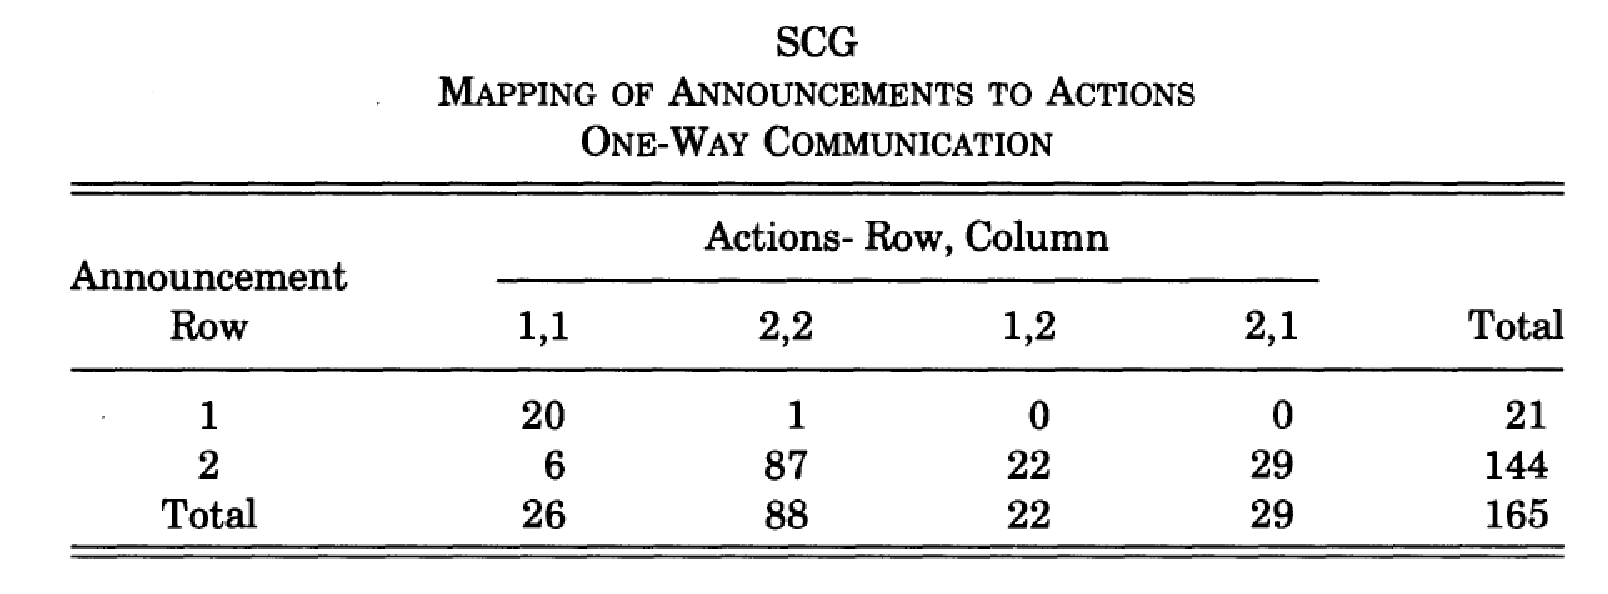
\includegraphics[width=0.95\textwidth]{./i/cdfr1992Tbl2.eps}\end{center}
\end{card}
\begin{card}
	\begin{itemize}
		\item Most messages are coordinating on the pareto-dominant symmetric equilibrium
		\item But those receiving messages only play strategy $2$  about 75\% of the time.
	\end{itemize}
\end{card}
\end{frame}

\begin{frame}{Cooper et al. (QJE 1992)}
\begin{card}
\begin{center}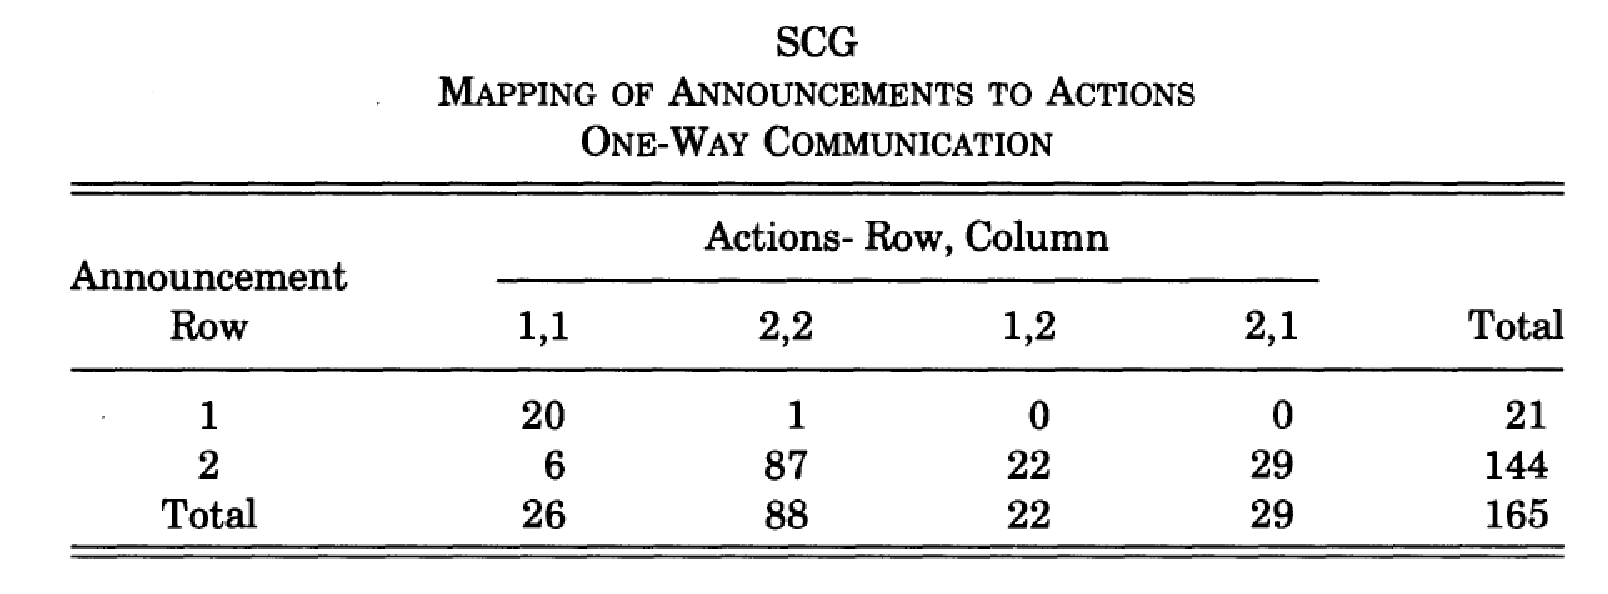
\includegraphics[width=0.9\textwidth]{./i/cdfr1992Tbl2.eps}\end{center}
\end{card}
\begin{card}
	\begin{itemize}
		\item Need greater than 80\% chance for a risk-nuetral agent to choose $2$
		\item Those sending $2$ choose that strategy 80.6\% of the time
	\end{itemize}
\end{card}
\end{frame}

\begin{frame}{Cooper et al. (QJE 1992)}
\begin{card}
\begin{center}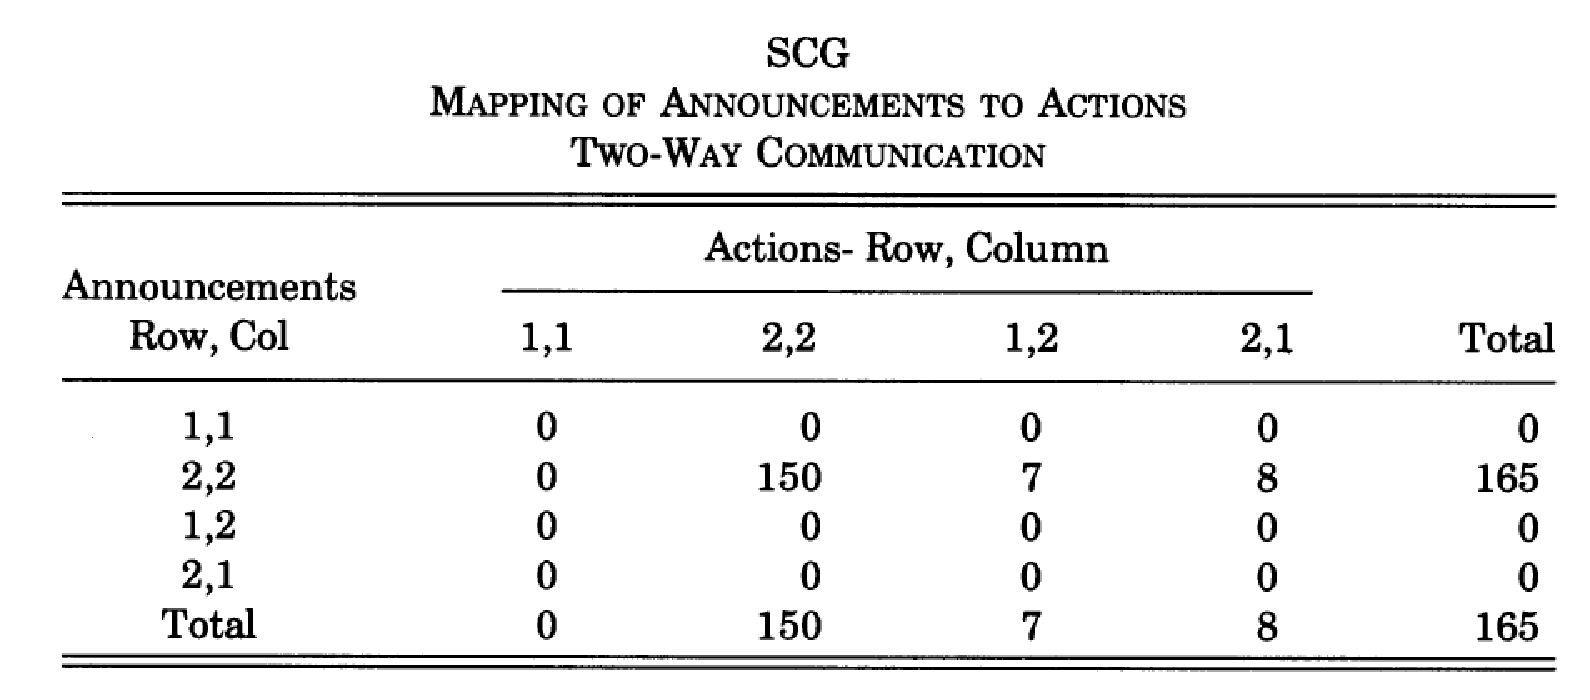
\includegraphics[width=0.8\textwidth]{./i/cdfr1992Tbl3.eps}\end{center}
\end{card}
    \begin{card}
    	\begin{itemize}
    		\item \textbf{All} messages are coordinating on the pareto-dominant symmetric equilibrium
    		\item 95.6\% of choice are for 2, with no outcomes at pareto-inferior equilibrium
    	\end{itemize}
    \end{card}
\end{frame}

\begin{frame}{Cooper et al. (QJE 1992)}
\begin{card}
\begin{center}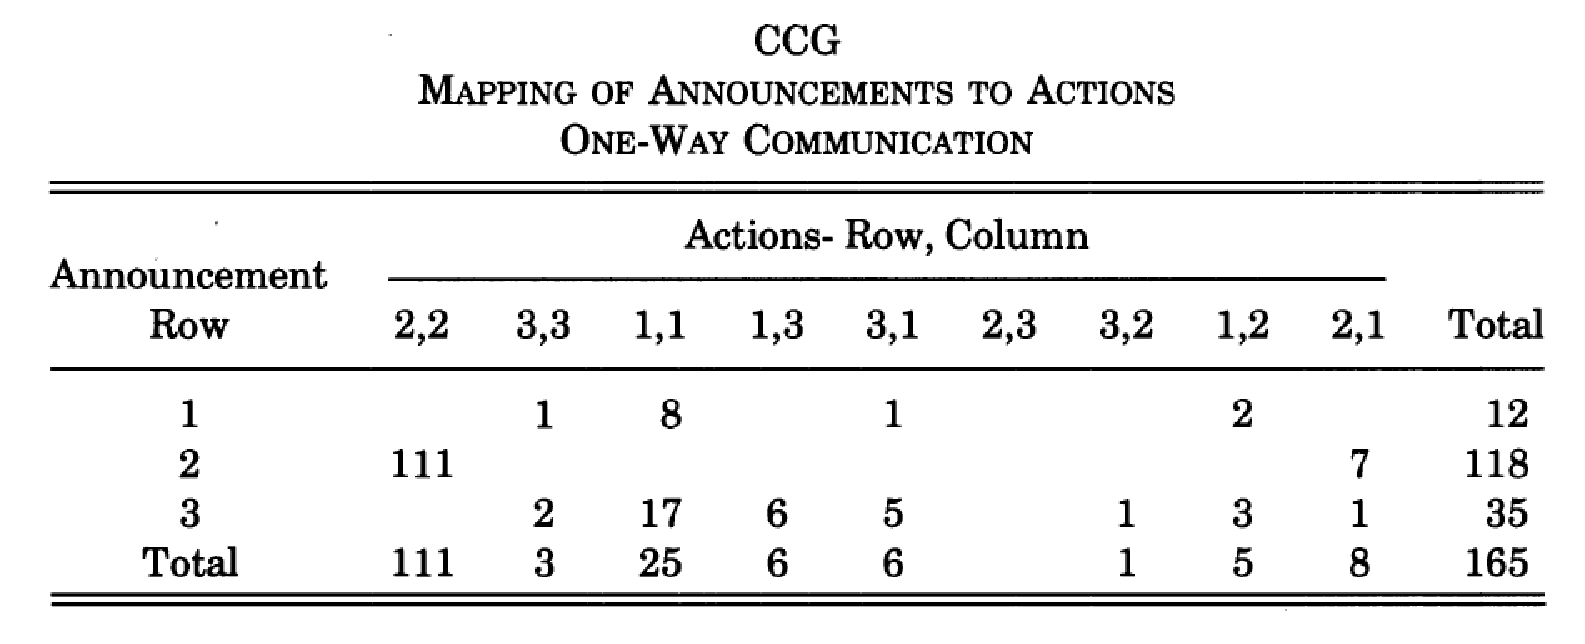
\includegraphics[width=0.8\textwidth]{./i/cdfr1992Tbl5.eps}\end{center}
\end{card}
\begin{card}
	\begin{itemize}
		\item 67.2\% of one-way messages are for the pareto-dominant equilibrium
		\item 94.1\% of the time yielding that outcome
		\item Messages for 3 are mostly fool's gold
	\end{itemize}
\end{card}
\end{frame}

\begin{frame}{Cooper et al. (QJE 1992)}
\begin{card}
\begin{center}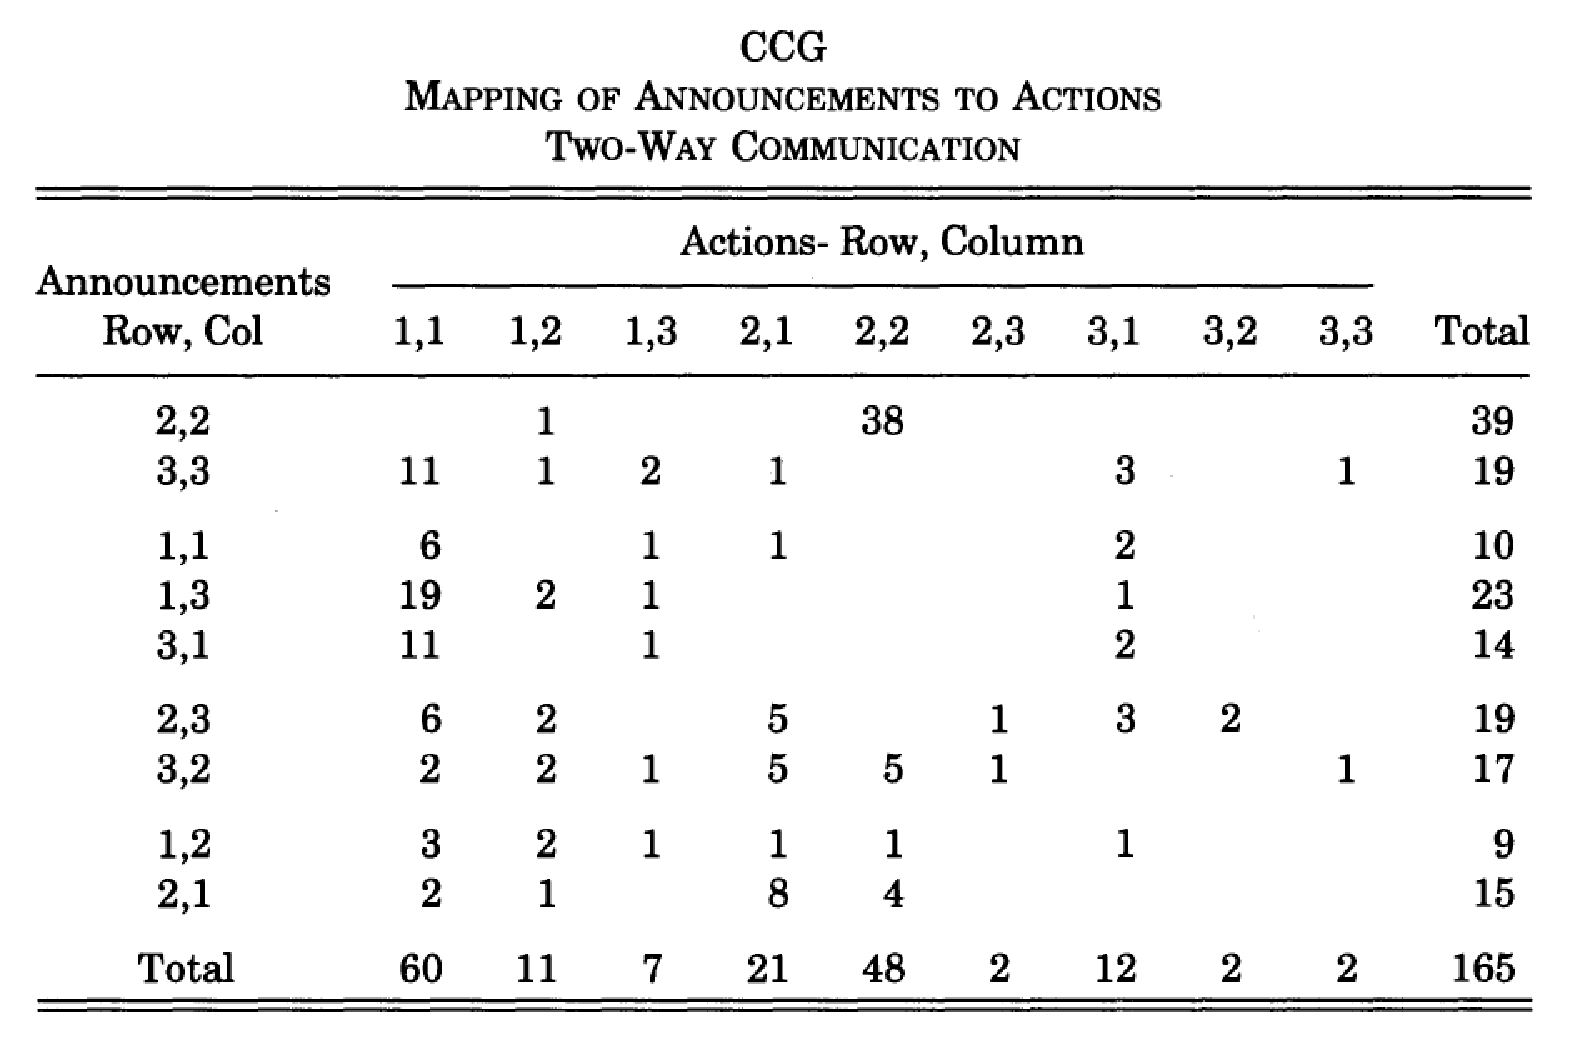
\includegraphics[width=0.6\textwidth]{./i/cdfr1992Tbl6.eps}\end{center}
\end{card}
\begin{card}
	\begin{itemize}
		\item $(2,2)$ announcements are great for coordinating (38/39)
		\item Messages \textbf{for} the cooperative outcome mostly yield the pareto-inferior equilibrium outcome
	\end{itemize}
	\end{card}
\end{frame}

\begin{frame}{Cooper et al. (QJE 1992)}
    \begin{card}
    	\begin{itemize}
    		\item Authors fit an explanatory model with ``altruists'' and ``egoists''
    		\item Binary model of other-regarding preference
    		\item Altruists want to play the (3,3) outcome, but egoists want the cash\pause
    		\item Communication that could allow equilibrium coordination gets co-opted for coordination in the prisoner's dilemma part \pause
    		\item Attempt to test model through selection of selfish or altruistic subjects from a dictator game (?). Mixed results for altrusits. Egoists are still selfish.
    	\end{itemize}
    \end{card}
\end{frame}

\begin{frame}{Duffy and Feltovich (2002)}
\begin{card}
 Primary motivation is coordination/efficiency, asking what coordination device is better:
	 \begin{itemize}
		 \item Cheap Talk
		 \item Observation
		 \item Experience
	\end{itemize}
\end{card}
\end{frame}


\begin{frame}{Duffy and Feltovich (2002)}
\begin{card}
\begin{center}
\begin{tabular}{r|c|c|}
				\multicolumn{1}{r}{}& \multicolumn{1}{c}{$C_2$}  & \multicolumn{1}{c}{$D_2$} \\ \cline{2-3}
				$C_1$ &  $70,70$ & $10,80$ \\ \cline{2-3}
				$D_1$ &  $80,10$ & $40,40$ \\ \cline{2-3}
\end{tabular}
\begin{tabular}{r|c|c|}
				\multicolumn{1}{r}{}& \multicolumn{1}{c}{$C_2$}  & \multicolumn{1}{c}{$D_2$} \\ \cline{2-3}
				$C_1$ &  $70,70$ & $10, 55$ \\ \cline{2-3}
				$D_1$ &  $55,10$ & $55,55$ \\ \cline{2-3}
\end{tabular}
\begin{tabular}{r|c|c|}
				\multicolumn{1}{r}{}& \multicolumn{1}{c}{$C_2$}  & \multicolumn{1}{c}{$D_2$} \\ \cline{2-3}
				$C_1$ &  $70,70$ & $50,80$ \\ \cline{2-3}
				$D_1$ &  $80,50$ & $40,40$ \\ \cline{2-3}
\end{tabular}
\end{center}
\end{card}

\end{frame}

\begin{frame}
\begin{card}[Within Treatment]
		\begin{itemize}
			\item Prisoner's Dilemma
			\item Stag Hunt
			\item Chicken
		\end{itemize}
\end{card}
\begin{card}[Between Treament]
		\begin{itemize}
			\item Cheap Talk
			\item Play Observation
			\item Nothing
		\end{itemize}
\end{card}
\end{frame}

\begin{frame}{Duffy and Feltovich (2002)}
\begin{card}
\begin{itemize}
	\item Lottery method, points are percentage chance of winning dollar
	\item Do not exhaust all within-subject orders (just run 2, SH in middle)
	\item 10 rounds each game
	\item 50-50 chance of being selected for treatment
\end{itemize}
\end{card}
\end{frame}


\begin{frame}{Duffy and Feltovich (2002)}
\begin{card}
\begin{center}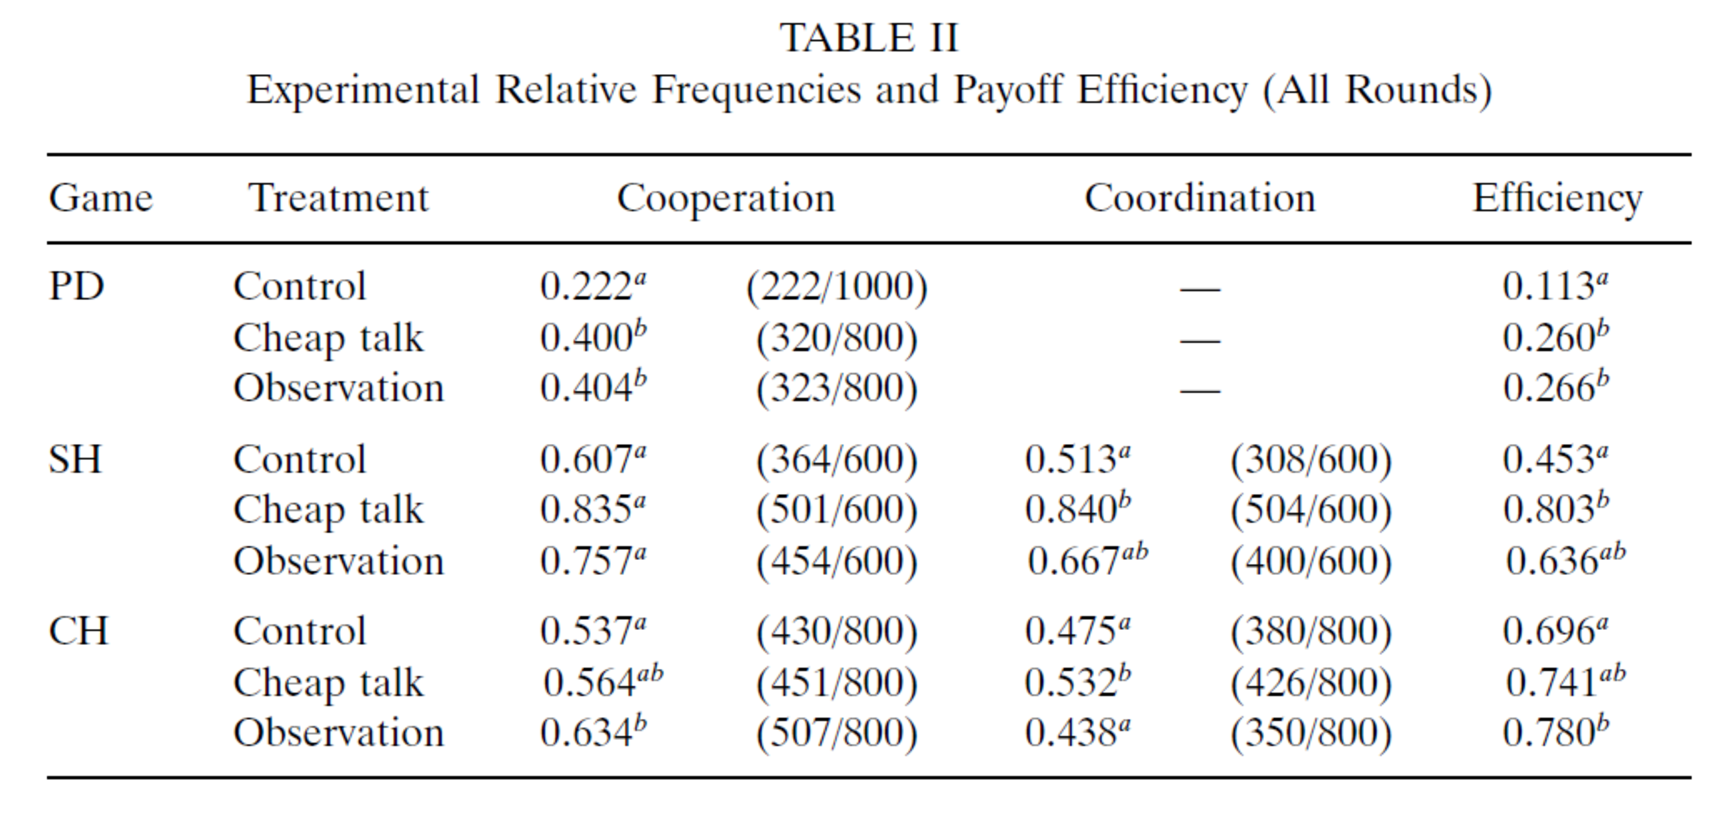
\includegraphics[width=0.99\textwidth]{./i/df2002tbl2.eps}\end{center}
\end{card}
\end{frame}

\begin{frame}{Duffy and Feltovich (2002)}
\begin{card}
\begin{center}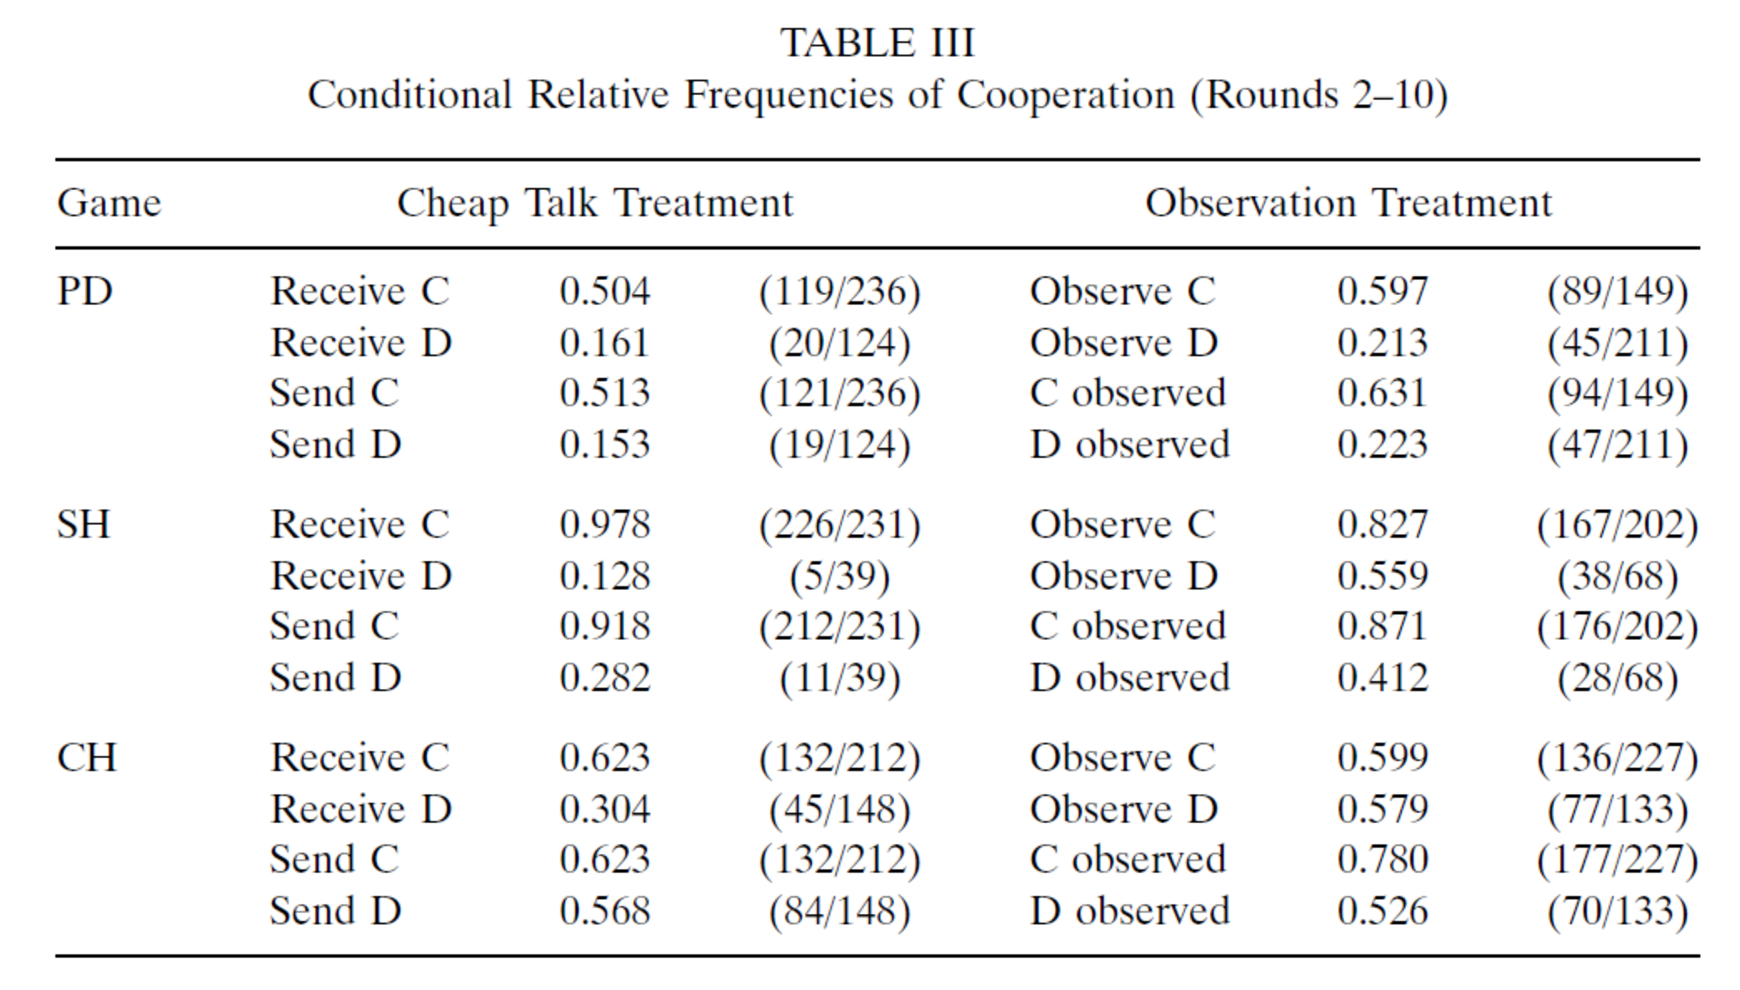
\includegraphics[width=0.9\textwidth]{./i/df2002tb3.eps}\end{center}
\end{card}
\end{frame}

\begin{frame}
\begin{card}[Conclusions]
\begin{itemize}
	\item Both observation and cheap talk are useful
	\item Cheap Talk better in games where common interest in coordination
	\item Observation better in PD and Chicken. (I would say this is more mixed)
\end{itemize}
\end{card}
\end{frame}

\begin{frame}{Spier and Landeo (AER 2009)}
\begin{card}
	\begin{itemize}
		\item Paper analyzes the `Naked Exclusion' model
		\item Monopolist offers exclusive dealing contracts to buyers.
		\item If the buyers can cooperate to both say no to monopolist, then a new entrant can profitable enter and reduce prices.
		\item But rejecting is risky, if there's no entrant you have to pay monopoly price, may be safer to take the monopolist's exclusive deal
	\end{itemize}
\end{card}
\end{frame}
\begin{frame}{Spier and Landeo (AER 2009)}
	\begin{itemize}
		\item The monopolist proposes an offer to each buyer $x_1$ and $x_2$
		\item Can either use a divide and conquer rule and give one player a dominant strategy to accept.
		\item Or can force the sellers into a stag-hunt coordination game
	\end{itemize}
\end{frame}

\begin{frame}{Spier and Landeo (AER 2009)}
\begin{card}
Sellers play a stag-hunt game which has payoffs:
	\begin{center}
		\begin{tabular}{r|c|c|}
			\multicolumn{1}{r}{} & \multicolumn{1}{c}{Accept} & \multicolumn{1}{c}{Reject} \\ \cline{2-3}
			$Accept$ &  $x_1,x_2$ & $x_1,0$  \\ \cline{2-3}
			$Reject$ &  $0,x_2$ & 1000,1000  \\ \cline{2-3}
		\end{tabular}
	\end{center}
\end{card}

\begin{card}
	\textbf{Question:} What is the effect of seller's possible communication on buyers' offers $(x_1,x_2)$?
\end{card}
\end{frame}

\begin{frame}
	\begin{card}[Treatments]
	Three variation dimensions in a factorial design
		\begin{enumerate}
			\item Communication or not between Buyers 
			
			(Simultaneous two-way)
			\item Exogenous or Endogenous offers 
			
			(Human/Robot buyer)
			\item Discrimination/No-discrimination between offers 
			
			($x_1=x_2$ or $x_1$ and $x_2$ independent offers)
		\end{enumerate}
	\end{card}
\end{frame}

\begin{frame}
\begin{card}[Exclusion rates]
\begin{tabular}{llcc}\toprule
		\multicolumn{1}{l}{Offers} & \multicolumn{1}{l}{ Discrim.} & \multicolumn{1}{c}{ No Comm.} & \multicolumn{1}{c}{Comm.} \\ \midrule
		Exogenous   & No    &  0.81 & 0.12  \\
		            & Yes   &  0.81 & 0.61  \\
		Endogenous  & No    &  0.92 & 0.43  \\
		            & Yes   &  0.82 & 0.79  \\ \bottomrule
	\end{tabular}
\end{card}
		\pause
\begin{card}
		\begin{itemize}
    		\item Offer asymmetry reduces efficacy of communication
		\end{itemize}
\end{card}
\end{frame}


\begin{frame}
\begin{card}[Discriminatory Offers]
	\begin{tabular}{lccccc}\toprule
			&  \multicolumn{2}{c}{Discr.} &\  & \multicolumn{2}{c}{No Discr.}\\\cline{2-3} \cline{5-6}
			\multicolumn{1}{l}{Offer}  & \multicolumn{1}{c}{No Comm} & \multicolumn{1}{c}{Comm}  & & \multicolumn{1}{c}{No Comm} & \multicolumn{1}{c}{Comm}\\ \midrule
			$(100,100)$  &  0\%  & 1.5\%  & & 4.2\%  & 7.5\% \\
			$(650,100)$  &  5.6\%  & 3.0\%  \\
			$(800,100)$  &  13.9\%  & 4.5\%  \\
			$(1100,100)$ &  57.6\%  & 85.6\% \\ 
			$(650,650)$  &  21.5\%  & 5.3\% & & 93.3\%  & 61.7\%  \\ 
			$(800,650)$  &  0.7\%  & 0\%  \\ 
			$(800,800)$  &  0.7\%  & 0\% & & 2.5\%  & 30.8\% \\ \bottomrule
		\end{tabular}
\end{card}
\end{frame}

\begin{frame}
\begin{card}[Exclusion Rates (Endogenous)]

	\begin{tabular}{lccccc}\toprule
			&  \multicolumn{2}{c}{Discr.} &\  & \multicolumn{2}{c}{No Discr.}\\\cline{2-3} \cline{5-6}
			\multicolumn{1}{l}{Offer}  & \multicolumn{1}{c}{No Comm} & \multicolumn{1}{c}{Comm}  & & \multicolumn{1}{c}{No Comm} & \multicolumn{1}{c}{Comm}\\ \midrule
			$(100,100)$  &  -  & 0\%  & & 0\%  &0\% \\
			$(650,100)$  &  25\%  & 25\%  \\
			$(800,100)$  &  25\%  & 0\%  \\
			$(1100,100)$ &  100\%  & 88\% \\ 
			$(650,650)$  &  84\%  & 43\% & & 96\%  & 39\%  \\ 
			$(800,650)$  &  100\%  & -  \\ 
			$(800,800)$  &  100\%  & - & & 100\%  & 59\% \\ \bottomrule
		\end{tabular}
\end{card}
\end{frame}

\begin{frame}
\begin{card}[Exclusion Rates (Exogenous)]
	\begin{tabular}{lccccc}\hline
			&  \multicolumn{2}{c}{Discr.} &\  & \multicolumn{2}{c}{No Discr.}\\\cline{2-3} \cline{5-6}
			\multicolumn{1}{l}{Offer}  & \multicolumn{1}{c}{No Comm} & \multicolumn{1}{c}{Comm}  & & \multicolumn{1}{c}{No Comm} & \multicolumn{1}{c}{Comm}\\ \hline
			$(100,100)$  &  -  & 50\%  & & 0\%  &0\% \\
			$(650,100)$  &  0\%  & 0\%  \\
			$(800,100)$  &  50\%  & 17\%  \\
			$(1100,100)$ &  99\%  & 69\% \\ 
			$(650,650)$  &  71\%  & 0\% & & 96\%  & 39\%  \\ 
			$(800,650)$  &  100\%  & -  \\ 
			$(800,800)$  &  100\%  & - & & 100\%  & 59\% \\ \hline
		\end{tabular}
\end{card}
\end{frame}

\begin{frame}{Coordination: Freeform Chat}
\begin{card}
    \begin{itemize}
    	\item The coordination papers we have examined here use very stylized message-spaces
    	\item More recent papers have instead focused on how free-form chat can solve this problem
    	\item In general, if you want to provide a \emph{very} strong coordination device, allowing the participants to chat is your best option
    	\item However, there are some cons:
    	\begin{itemize}
    		\item Reduce anonymity
    		\item Increased appeals to what is fair
    	\end{itemize}
    	\item I'll come back to this at the end of the next section.
    \end{itemize}
\end{card}

\end{frame}
\end{document}
